\begingroup
	\pgfdeclarelayer{lineas}
	\pgfdeclarelayer{dibujo}
	\pgfsetlayers{lineas, dibujo, main}
	\tikzstyle{one}=[circle,draw=black,fill=black,inner sep=0pt,minimum size=2.5mm]
	\tikzstyle{two}=[circle,draw=black,fill=white,inner sep=0pt,minimum size=2.5mm]
	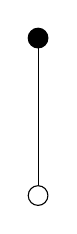
\begin{tikzpicture}	
		\node at (1.732,1) [one] {};
		\node at (1.732,-1) [two] {};			
		
		\begin{pgfonlayer}{dibujo}
			\draw (1.732,1)--(1.732,-1);
		\end{pgfonlayer}
	\end{tikzpicture}
	%\label{fig:1_simplex}
\endgroup
\endinput